\chapter{Espace aérien, trafic, Vol en équipe}\label{cha:airspace}
Les données spécifiques à l'utilisation de l'espace aérien (SUA pour Special Use Airspace) peuvent être chargées dans XCSoar. Elles sont utilisées pour l'affichage des différents types d'espaces et pour la détection de l'entrée/sortie de l'aéronef dans ces espaces.

Deux fichiers d'espaces aériens peuvent être référencés. Le premier est la base de donnée SUA principale, le second est dédié aux espaces changeants fréquemment (valables sur une courte période) comme les espaces concernés par des NOTAM.

Il est de la responsabilité de l'utilisateur de s'assurer que les données relatives aux espaces aériens (fichiers espaces aérien et autres esp. aér.) sont à jour.

A l'aide d'un FLARM connecté, le calculateur affiche aussi les informations des autres aéronefs des environs, équipés de FLARM.

Une fonctionnalité "Code équipe" permet à des équipes de pilotes d'échanger leurs positions par radio en utilisant un code qui ne peut signifier quelque chose que pour leurs coéquipiers. Ces données sont encodées et décodées par le calculateur.

\section{Affichage des espaces aériens}
Les espaces aériens (SUA) sont représentés par une zone hachurée avec une bordure épaisse. La couleur est spécifique au type d'espace et peut-être configurée par l'utilisateur. En fonction du paramétrage, il est possible d'afficher tout les espaces, seulement ceux sous une certaine altitude, seulement ceux compris entre deux altitudes ou bien seulement ceux qui sont sous le planeur.  
\sketch{figures/airspace.png}

Les modèles de représentation peuvent être opaques, transparents au milieu, hachurés  continus ou pointillés. Les modèles non-opaques sont partiellement transparents en ce qui concerne le relief et la topographie, mais ne sont pas transparents pour les espaces aériens se chevauchant. Cependant, quand des espaces se chevauchent leurs bordures sont affichées. C'est-à-dire que pour les modèles d'espace aérien qui ne sont pas mutuellement transparents, toutes les frontières d'espace aérien sont dessinées au-dessus des zones d'espace aérien.

L'affichage et l'alerte de pénétration d'une classe peuvent être activé ou désactivé, individuellement, par l'utilisateur. Voir la section~\ref{sec:airspacedetails}.

Les couleurs par défaut des classes C, D, E et F sont conformes aux cartes OACI.


\subsection*{Événements d'intrusion}

3 types d'événements sont détectés par XCSoar concernant les espaces aériens (SUA) :
\begin{description}
\item[Incursion Prévue] Cet évènement est levé quand la trajectoire du planeur est estimée entrer dans l'espace aérien dans un laps de temps paramétrable. Ce laps de temps est le "Temps d'alerte" du menu de configuration.

Les calculs utilisent la moyenne de la direction de la trajectoire sur une période de temps longue: ceci permet de prédire l'incursion dans une zone même en spirale quand le planeur dérive, du fait du vent.


%{\it DIAGRAM SHOWING DETECTION OF PREDICTED INCUSION WHEN CIRCLING AND
%  CRUISING}

\item[Entrée] Évènement levé lors de l'entrée dans un espace aérien.
\item[Sortie] Évènement levé lors de la sortie d'un espace aérien.
\end{description}
En toutes circonstances, le pourtour de l'espace est défini par les altitudes mini et maxi ou par les niveaux de vol définis dans le fichier des espaces aériens.

Les alertes d'incursion dans un espace aérien sont levées même si le lieu de pénétration dans la zone est en dehors de l'écran.

Quand l'altitude provient d'un altimètre barométrique, celui-ci est utilisé à la place de l'altitude fournie par le GPS, lors du calcul d'intrusion dans les espaces aériens. Ceci rend le système conforme aux conventions de calcul de violation des espaces aériens, basé sur le QNH.

\section{Alertes et espaces aériens}

Introduction du concept de niveau graduel des alertes d'espaces aériens :
\begin{description}
\item[Aucune] L'aéronef est à l'extérieur et à une certaine distance de tout espace aérien.
\item[\colorbox{AirspaceYellow}{Near}] L'aéronef se rapproche et va bientôt entrer dans un espace aérien.
\item[\colorbox{AirspaceRed}{Inside}] L'aéronef est à l'intérieur d'un espace aérien.
\end{description}

En permanence, XCSoar contrôle la position de l'aéronef par rapport à tous les espaces aériens du fichier d'espaces aériens et gère les niveaux d'alertes pour chaque espace. Les alertes sont filtrées en accord avec les préférences définies par l'utilisateur: ainsi certains types d'espaces peuvent être totalement ignorés.
\sketch{figures/airspacewarning.png}
La séquence des évènements levés en entrant dans une zone est constituée de deux alertes : niveau 1 = proche = "near" et niveau 2 = à l'intérieur = "inside".

A chaque accroissement du niveau d'alerte ( supérieur à 0 ) quelque soit l'espace, la boite de dialogue s'affiche avec un bip sonore. Quand il n'y a plus d'espace ayant un niveau d'alerte au dessus de 0, la boite de dialogue se ferme automatiquement.

\subsection*{La boite Alertes Airspace}

La boite de dialogue "Alertes Airspace" peut comporter jusqu'à quatre alertes individuelles. Le bouton est rouge pour signifier que l'aéronef est dans la zone, jaune si il en est proche et une alerte qui a été reconnue est écrite en gris.

Chaque alerte occupe 2 lignes et comporte les détails suivants :\\ 
\verb+<NOM et Classe>   <NIVEAU SUP.>  <Niveau Alerte>+  \\
\verb+<Temps et distance si à l'extérieur> <NIVEAU INF.>+

Les alertes du panel sont mises à jour continuellement.
Voici un exemple :\\
\verb+ECRINS 1000m/sol No (1000 m    AGL  +\colorbox{AirspaceYellow}{near} \\
\verb+30 sec dist 2130 m             GND+

Ce qui signifie que l'aéronef est à 30 secondes environ et 2130 m horizontalement de la bordure de la zone des ECRINS. survol interdit au dessous de 1000 m sol.

Un autre exemple :\\
\verb+R196A1 Est GAP (Notam         FL195  + \colorbox{AirspaceRed}{inside}  \\
\verb+                     1006 m   AGL+

Signifie que l'aéronef est dans la zone R196A1 de plafond FL 195 et de base 1006 m sol. Cette zone étant spécifiée par NOTAM (Zone de parachutage au-dessus de GAP).

A chaque alerte d'espace aérien, la boite de dialogue s'ouvre et vous pouvez avoir les détails de la zone en question, en appuyant dessus (Pour Altair il faut sélectionner et appuyer sur Enter).
\begin{center}
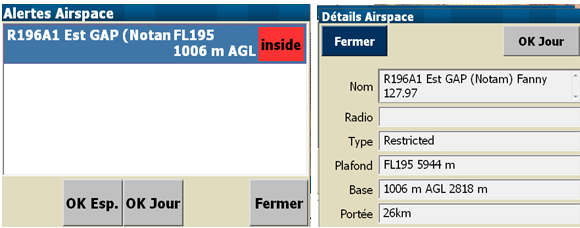
\includegraphics[angle=0,width=\linewidth,keepaspectratio='true']{figures/alerteespaceaerien2.png}
\end{center}


\subsection*{Accusé de réception des alertes}

Quand la boite de dialogue des alertes est ouverte et qu'une alerte est active, la boite peut-être fermée ( sur PC en appuyant sur Echap. ) ou sur  \bmenug{Fermer}. Ceci ferme la boite sans accuser la réception de l'alerte.

Quand une ou plusieurs alertes sont vivibles dans la boite de dialogue des alertes, une alerte peut peut être validée en appuyant sur l'un des boutons au bas de la boite. Si la liste comporte plusieurs alertes, le bouton rotatif sur Altair, le curseur sur PDA ou le doigt sur Androïd permettent de sélectionner l'alerte à valider.

Signification des boutons de validation  des alertes :
\begin{description}
\item[OK Alert.]  Accuse réception du niveau de l'alerte courant. Une nouvelle alerte apparaitra seulement si le niveau d'alerte augmente. (touche F5 sur Altair) 
\item[OK Esp.]  Accuse réception de tout les niveaux d'alerte courants et futurs concernant cet espace aérien, et ceci tant qu'il est éloigné à moins de 2,5 km horizontalement et 500m verticalement. (touche F6 sur Altair)  
\item[OK Jour]  Accuse réception de tout les niveaux d'alerte courants et futurs concernant cet espace aérien pour le reste du vol. (touche F5 sur Altair) . Sur Altair, si XCSoar est redémarré, cet accusé de réception n'est plus valable.
\item[Activer]  Invalide un accusé de réception d'un espace aérien et ré-active les alertes de cet espace. (touche F8 sur Altair) 
\item[Fermer] Ferme la boite de dialogue des alertes, sans accuser réception des alertes levées. La boite de dialogue s'ouvre à nouveau automatiquement si le niveau d'alerte augmente.
\end{description}

Remarque : les différents boutons ne sont pas tous visibles pour tous les niveaux d'alerte. En particulier, si à l'intérieur d'un SUA, le bouton  \bmenug{OK Alert.} n'apparait pas, cela signifie que l'espace concerné n'est plus une menace imminente mais que vous y avez déjà pénétré. 

Règles générales d'utilisation de la boite de dialogue des alertes :
\begin{itemize}
\item  Ne pas accuser réception d'une alerte qui concerne un espace que vous devez contourner.
\item  Le bip de l'alerte est seulement émis lors de l'accroissement du niveau de l'alerte.
\item  Le système d'alerte est conçu pour permettre de spiraler près d'un espace aérien sans stresser inutilement  le pilote en générant des alarmes en trop.
\end{itemize}

Quand on accuse réception pour un espace aérien avec \bmenug{OK Esp.}, il n'est plus représenté que par son pourtour, les hachures sont supprimées.

Quand il va y avoir pénétration dans un espace aérien ou qu'il y a déjà pénétration, une alarme sonore est émise avec un message détaillé décrivant le type d'espace ( classe, plancher et plafond en altitude ou niveaux de vol).

Les alertes ayant été acquittées sont répétées après un certain temps qui est configurable dans le menu Option Système sous le nom : "Temps d'acquittement".

L'acquittement d'une alerte ne s'applique qu'à un espace aérien donné. Si un planeur entre dans l'espace A et que le pilote accuse réception de cette alerte et qu'en même temps il s'approche aussi d'un autre espace B, une alerte sera levée concernant l'espace B.

\tip Si vous souhaitez que les alertes acquittées soient répétées, il est conseillé de mettre une grande valeur au paramètre  "Temps d'acquittement".

Les alertes, concernant un espace, sont effacées de la boite de dialogue quand la position du planeur ainsi que sa trajectoire future estimée sont en dehors de l'espace considéré.

Plusieurs alertes peuvent être déclenchées simultanément si l'aéronef (ou sa trajectoire estimée) pénètre dans plusieurs espaces.

\section{Recherche et détails des espaces}\label{sec:airspacedetails}

Pour les terminaux "touchscreen" ou ayant une souris, si un espace aérien est visible sur la carte, il suffit de le toucher ou de cliquer dessus pour obtenir les détails le concernant. La liste des éléments de la carte apparait et donne un aperçu des points de virages, terrains, position actuelle et espaces aériens qui sont à l'endroit sélectionné. Les espaces aériens sont affichés de la même façon que lors des alertes. La recherche donne tous les espaces aériens visibles sur la carte qui se chevauchent à l'endroit sélectionné.
\sketch{figures/airspace_mapelements.png}
Le fait de sélectionner un espace aérien dans la liste et d'appuyer sur \button{Détails} permet de voir tous les détails concernant l'espace choisi.

\tip Une autre façon de rechercher les espaces aériens et autres informations : en mode PAN ON (panoramique), déplacer la carte pour positionner le curseur à l'endroit désiré.  Appuyer sur le bouton  \button{Qu'y a-t-il ici??} pour afficher la même liste des éléments de la carte à cet endroit.



\subsection*{Recherche et filtrage des espaces aériens}\label{sec:airspace-filter}

La boite de dialogue de filtrage des espaces aériens permet de d'activer ou non les alertes et l'affichage de chaque classe d'espace.

On y accède de plusieurs manières :
\begin{itemize}
\item Du menu principal \bmenug{Config. 2}\blink\bmenug{Régl. Esp. Aériens}.
\item Du menu Espace aérien dans Options Système, en appuyant sur \button{Filtre}.
\end{itemize}

\sketch{figures/airspacefilter.png}
Pour utiliser cette boite de dialogue, sélectionner une classe : à chaque pression la configuration change en permettant l'affichage de l'espace uniquement, de l'alerte uniquement, ni l'un ni l'autre ou bien les 2. (la touche Enter fait de même).

\subsection*{Gestion des espaces aériens}

En appuyant sur \button{Parcourir} la boite de dialogue de gestion des espaces aérien apparait.  Sont utilisation est similaire à celle de la boite de dialogue de gestion des points de virage. Il est possible de rechercher sur les critères de nom, de distance de cap et de type (classe).
\sketch{figures/airspacelookup.png}

Quand l'espace aérien est trouvé, il est possible de l'acquitter pour la journée ou de l'activer si il ne l'était plus.

\section{Analyses}

L'une des pages de la boite de dialogue Analyses montre une coupe verticale de l'espace aérien. On y accède par :
\begin{quote}
\bmenug{Info. 1}\blink\bmenug{Analyses}
\end{quote}

Cette section montre les 50 km de l'espace aérien dans la direction du planeur (axe des X) et son altitude ( axe des Y ). L'altitude du planeur est indiquée par un flèche sur la gauche. Cette page est très utile pour visualiser l'imbrication des espaces aériens, qui peut être complexe dans certaines situations.

\begin{center}
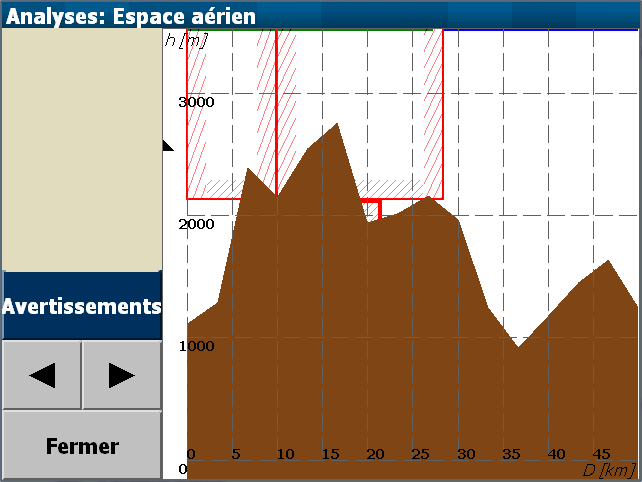
\includegraphics[angle=0,width=0.8\linewidth,keepaspectratio='true']{figures/analysis-airspace.png}
\end{center}

Le bouton "Avertissements" ouvre directement la page des alertes quand le planeur est à proximité ou à l'intrieur d'un espace aérien.
\begin{center}
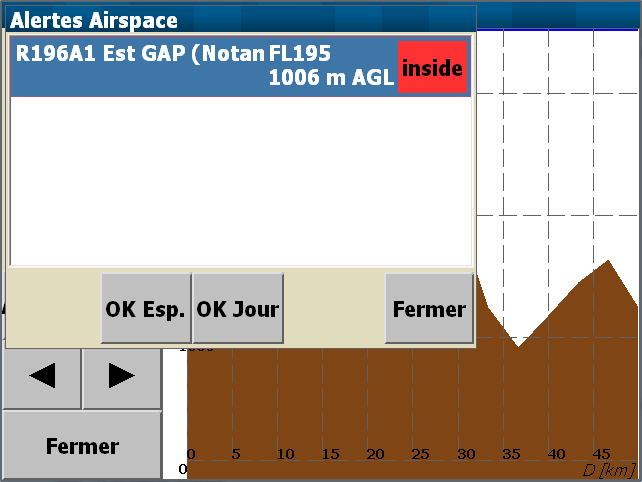
\includegraphics[angle=0,width=0.8\linewidth,keepaspectratio='true']{figures/analysis-airspace2.png}
\end{center}


\section{Trafic et FLARM}

Si XCSoar est connecté à un FLARM, les planeurs équipés d'un FLARM sont visibles sur la carte. Chaque aéronef qui est reçu, est représenté par un cercle rouge en pointillés.

\warning Il ne faut pas utliser XCSoar en tant qu'anti-collision. Le FLARM est une aide et est la référence. Il ne doit pas empêcher de regarder dehors!!!

Remarque : à moins de spiraler, le niveau de zoom ne permet pas de distinguer aisément les autres FLARMs dans le secteur. En spirale le niveau de zoom peut-être correct, mais le changement constant de cap et la latence du PDA font que l'aide à la localisation des autres aéronefs n'est pas très efficace et fiable.

\subsection*{Affichage du trafic sur la carte}

Les cibles FLARM sur la carte sont représentées par des flèches rouges dont la pointe montre la direction de l'aéronef ayant un FLARM ainsi que le risque\config{flarm-on-map} de collision. Notez que l'orientation des flèches dépend du mode d'affichage de la carte. Par exemple, si le mode d'affichage est "Route en haut", les flèches pointent vers la direction relative des cibles par rapport au planeur. Si le mode d'affichage est "Nord en haut", les flèches pointent vers la direction des routes absolues des cibles.
\sketch{figures/flarmmap.png}

L'affichage sur la carte des données d'identification des FLARMs (numéro de concours, nom du piilote, immatriculation) est possible par l'intermédiaire d'un fichier OACI d'identification de trafic aérien pour FLARM : voir section~\ref{sec:flarm-ident-file} pour plus de détails sur le format du fichier. Les aéronefs ayant activé l'option "anonyme" de leur FLARM ne seront identifiés que par une flèche, aucune donnée d'identification ne sera affichée.

\subsection*{Radar FLARM}

Pour palier à cette situation, quand un trafic FLARM est reçu, XCSoar affiche une petite fenêtre de type FLARM du point de vue de l'aéronef. Le trafic FLARM est représenté de la même façon, mais les cibles menaçantes sont rendues plus visibles en étant entourées de un ou deux cercles. Le coin d'affichage de cette vue radar FLARM peut-être paramétré, voir \config{flarmradar-place}.

Cette vue de radar FLARM est affichée en mode "Route en haut" et un petit planeur, au centre, rappelle ce mode d'affichage. L'échelle est linéaire jusqu'à 2 000 mètres. En fond d'écran il y a 2 cercles : le premier a un rayon de 1 000 m et le second 2 000 m. Le trafic distant de plus de 2 km du centre est représenté sur le cercle des 2 km.
\sketch{figures/flarmrose.png}

Tout les affichages du trafic FLARM montrent le trafic avec les mêmes couleurs, symbolisant la menace potentielle ou le vol en équipe. Les couleurs sont :
\begin{itemize}
\definecolor{warning}{rgb}{1,0.64,0}
\definecolor{teammate}{rgb}{0.45,1,0}
\item \textcolor{black} {Noir pour le niveau 0, pas de danger.} 
\item \textcolor{warning} { Jaune pour le niveau 1, warning.}
\item \textcolor{red} {rouge pour les niveaux 2 et 3, alerte.}
\item \textcolor{teammate} {Vert pour le membre de l'équipe.}
\item \textcolor{blue} {Bleu pour la cible choisie.}
\end{itemize}

Pour toute cible dont la menace est supérieure à 1, la différence d'altitude arrondie est affichée. L'affichage montre la différence d'altitude arrondie à 100. Un petit triangle noir (au-dessus du 1 sur la figure) indique si la cible est au-dessus ou au-dessous de vous. L'exemple ci-dessous montre une cible environ 100 m au-dessus (pour une altitude en mètres) car il pointe vers le haut. 

Si activé, l'affichage de type radar FLARM peut-être supprimé en appuyant sur Fermer ou Enter suivant les plateformes (la molette sur Altair). La même action permet de ré afficher le radar. Quand une nouvelle cible apparait, ou si le radar emet une alerte de collision, l'affichage est automatique.

\subsection*{Interface graphique du trafic FLARM}\label{sec:flarm-traffic}

Dés que le FLARM détecte une cible et que la petite vue du radar apparait\config{flarmdisplay} vous pouvez appuyez dessus pour la mettre plein écran. Ceci peut aussi se faire par le menu \bmenug{Info. 1}\blink\bmenug{FLARM Radar}.
L'affichage plein écran offre toutes les informations concernant le trafic détecté par la FLARM. Suivant le paramétrage, il disparait automatiquement quand il n'y a plus de cible aux alentours.

\begin{center}
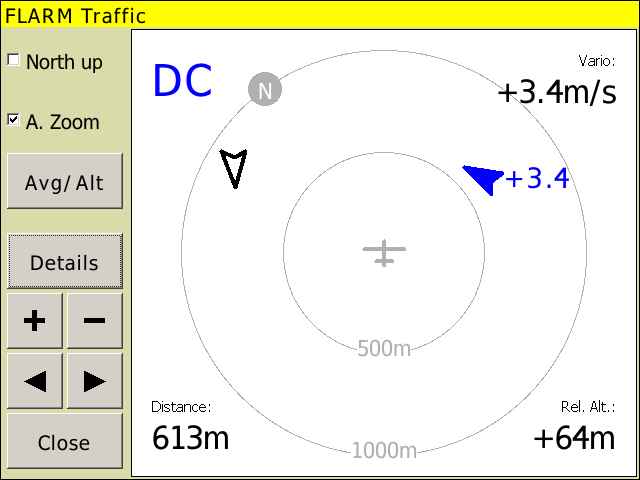
\includegraphics[angle=0,width=0.8\linewidth,keepaspectratio='true']{figures/dialog-flarm1.png}
\end{center}

Les boutons de contrôle de haut en bas :
\begin{description}
\item[Nord en haut]  Si coché, l'affichage est en mode "Nord en haut". Sinon, par défaut, c'est "Route en haut".
\item[A. Zoom]  \gesture{Haut - Bas} Réglage automatique du zoom pur que les cibles soient parfaitement visibles. Si pas coché, le zoom doit être ajusté manuellement. Le geste Haut - Bas passe en zoom automatique.
\item[Avg/Alt]  \gesture{Droite - Gauche} Bascule de l'affichage entre vario moyen et altitude moyenne à côté de la cible.
\item[Détails]  \gesture{Bas - Droit} A l'aide du bouton, une boite de dialogue concernant la cible choisie apparait, montrant tous les détails.
\item[+/-]  \gesture{Haut/Bas} Change manuellement le zoom de 500 m à 1000 m. Les commandes par gestes sont toujours possibles.
\item[$\triangleleft$/$\triangleright$]  \gesture{Gauche/Droite} Passage d'une cible à l'autre.
\end{description}

\begin{center}
\begin{tabular}{c c}
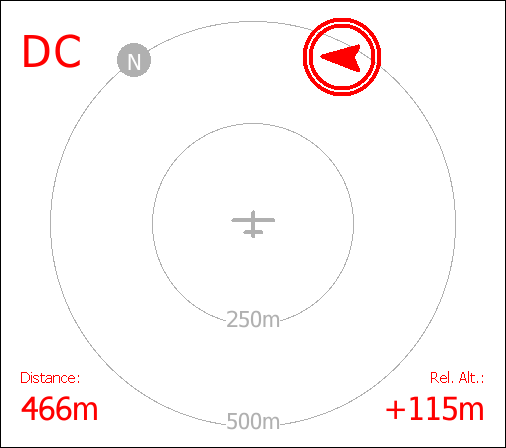
\includegraphics[angle=0,width=0.5\linewidth,keepaspectratio='true']{figures/cut-flarm2.png}&
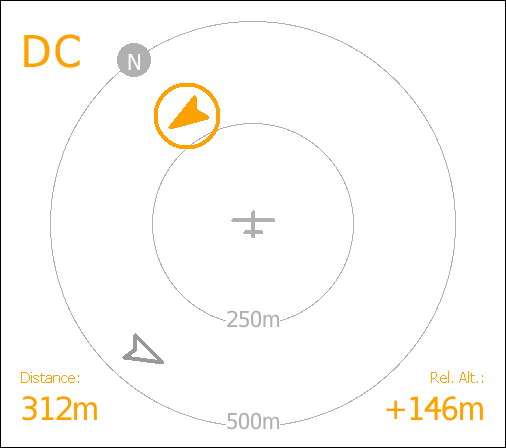
\includegraphics[angle=0,width=0.5\linewidth,keepaspectratio='true']{figures/cut-flarm3.png}\\
\end{tabular}
\end{center}
Les trois copies d'écran, prises en séquence, montrent le passage à proximité de 2 planeurs équipés de FLARM. Les informations détaillées sont en couleur et suivent le code de couleur décrit plus haut. 
Dans les 4 coins de l'écran radar les informations concernent la cible sélectionnée (si plusieurs cibles dans le secteur) :
\begin{description}
\item[Haut gauche]  Si disponible, identifiant FLARM de la cible sélectionnée.
\item[Haut droite]  Vario de la cible en moyennant les différentes altitudes reçues.
\item[Bas gauche]  Distance à la cible.
\item[Bas droite]  différence d'altitude entre l'aéronef et la cible. 
\end{description}

Entre la première et la seconde copie d'écran, 15 secondes sont passées. La cible bleue sélectionnée montait à +3,4 m/s et ne constituait pas une menace de collision envers le planeur. Pendant ce temps, le 'DC' s'est incliné vers la gauche, devenant une menace et passant alors en rouge. Le zoom du radar FLARM est alors passé de 1000m à 500m. La dernière copie d'écran montre que le 'DC' est en montée permanente, le niveau de "menace" est passé à 1, l'affichage est devenu orange.

\section{Vol en équipe}\label{sec:team-flying}

Le code équipe est un moyen, donné aux pilotes d'une équipe, de communiquer entre eux leur position de façon concise et avec précision. Le principe est que chaque pilote calcule un code à 5 caractères à l'aide du calculateur décrivant sa position par rapport à un point de virage commun à toute l'équipe. Les pilotes s'échangent leur codes par radio, et en entrant ces codes, ils peuvent visualiser leur équipiers sur la carte, avec précision.

Pour générer un code équipe, tous les pilotes doivent choisir un point de virage commun, qui est leur référence. Ceci se fait avec le panel "code équipe" \bmenug{Info. 2}\blink\bmenug{Equipe}. Le point de virage de référence est défini à l'aide du bouton \button{Def WP}. Le point de virage sélectionné dans la liste sera le point de virage de référence, devant être le même pour tous.

En vol le pilote peut donner son code équipe, personnel, à son équipier, à l'aide du panel "code équipe", afin de donner sa position de façon cryptée. Quand il entend le code d'un équipier, il appuie sur \button{Définir code} pour entrer ce code.\sketch{figures/dialog-teamcode.png}


Après avoir entré le code de son équipier, la distance entre les 2 planeurs est affichée ainsi que le cap à suivre pour rejoindre l'équipier. Ces valeurs sont mises à jour dans le panel.

XCSoar supporte aussi les codes d'équipe cryptés du projet FlarmNet. Le bouton \button{Capture Flarm ???} permet d'accéder à la base de données FlarmNet ainsi qu'aux données FLARM de XCSoar pour trouver un équipier. Une consultation simple???????????????? mais ambiguë d'un numéro de concours donne un identifiant FLARM, qui permet de localiser et de garder en permanence la position de l'équipier. Voir la section~\ref{sec:flarm-ident-file} pour plus de détails.

Enfin, XCSoar ne gère qu'un seul équipier avec un point de virage prédéfini, mais n'est pas limité en nombre de "copains" dont vous connaissez l'identifiant FLARM. Si vous vous rapprochez de vos collègues de vol, associez à chacun une couleur dans le panel de dialogue du FLARM et identifiez les à l'avenir en tant que copains.


\todo{flarm detail dialog}

